\section{Программный пакет \texttt{NuPropagator}}

\subsection{Общее описание и структура}

Пакет \texttt{NuPropagator}~\cite{nupropagator2022} представляет собой модуль для моделирования прохождения потоков нейтрино через вещество, в частности через Землю, с учётом взаимодействий по заряженному и нейтральному токам. Он реализует итеративный метод на основе $\mathcal{Z}$-фактора, что позволяет учитывать регенерацию нейтрино при рассеянии на нуклонах. Пакет написан на языке \texttt{Python3} и поддерживается через платформу \texttt{PyPI}, что обеспечивает его доступность и простоту интеграции в существующие симуляционные цепочки.

\begin{figure}[!h]
\centering
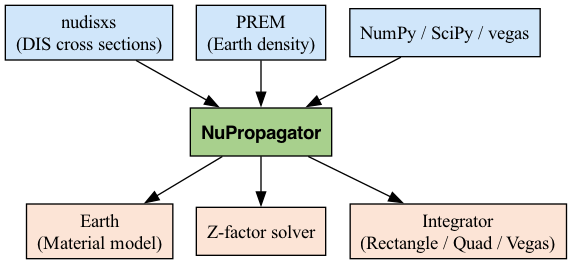
\includegraphics[width=\linewidth]{images/nupropagator_diagram.png}
\caption{Структура программного пакета \texttt{nupropagator} и его зависимости.}
\label{fig:nupropagator1}
\end{figure}

\subsection{Физическая модель}

Пакет \texttt{NuPropagator} использует следующие физические компоненты:
\begin{itemize}
  \item модель плотности Земли (PREM);
  \item сечения взаимодействия нейтрино с нуклонами, предоставляемые пакетом \texttt{nudisxs};
  \item итерационный метод Z-фактора для расчёта эволюции нейтринного спектра.
\end{itemize}

\subsection{Модель плотности Земли и расчёт толщины}

В качестве модели плотности используется Предварительная эталонная модель Земли (PREM)~\cite{dziewonskiPREM1981}, которая предполагает сферическую симметрию и описывает плотность, давление и другие параметры как функции радиуса. Плотность в модели представлена на рис.~\ref{PREM}.

\begin{figure}[!h]
\centering
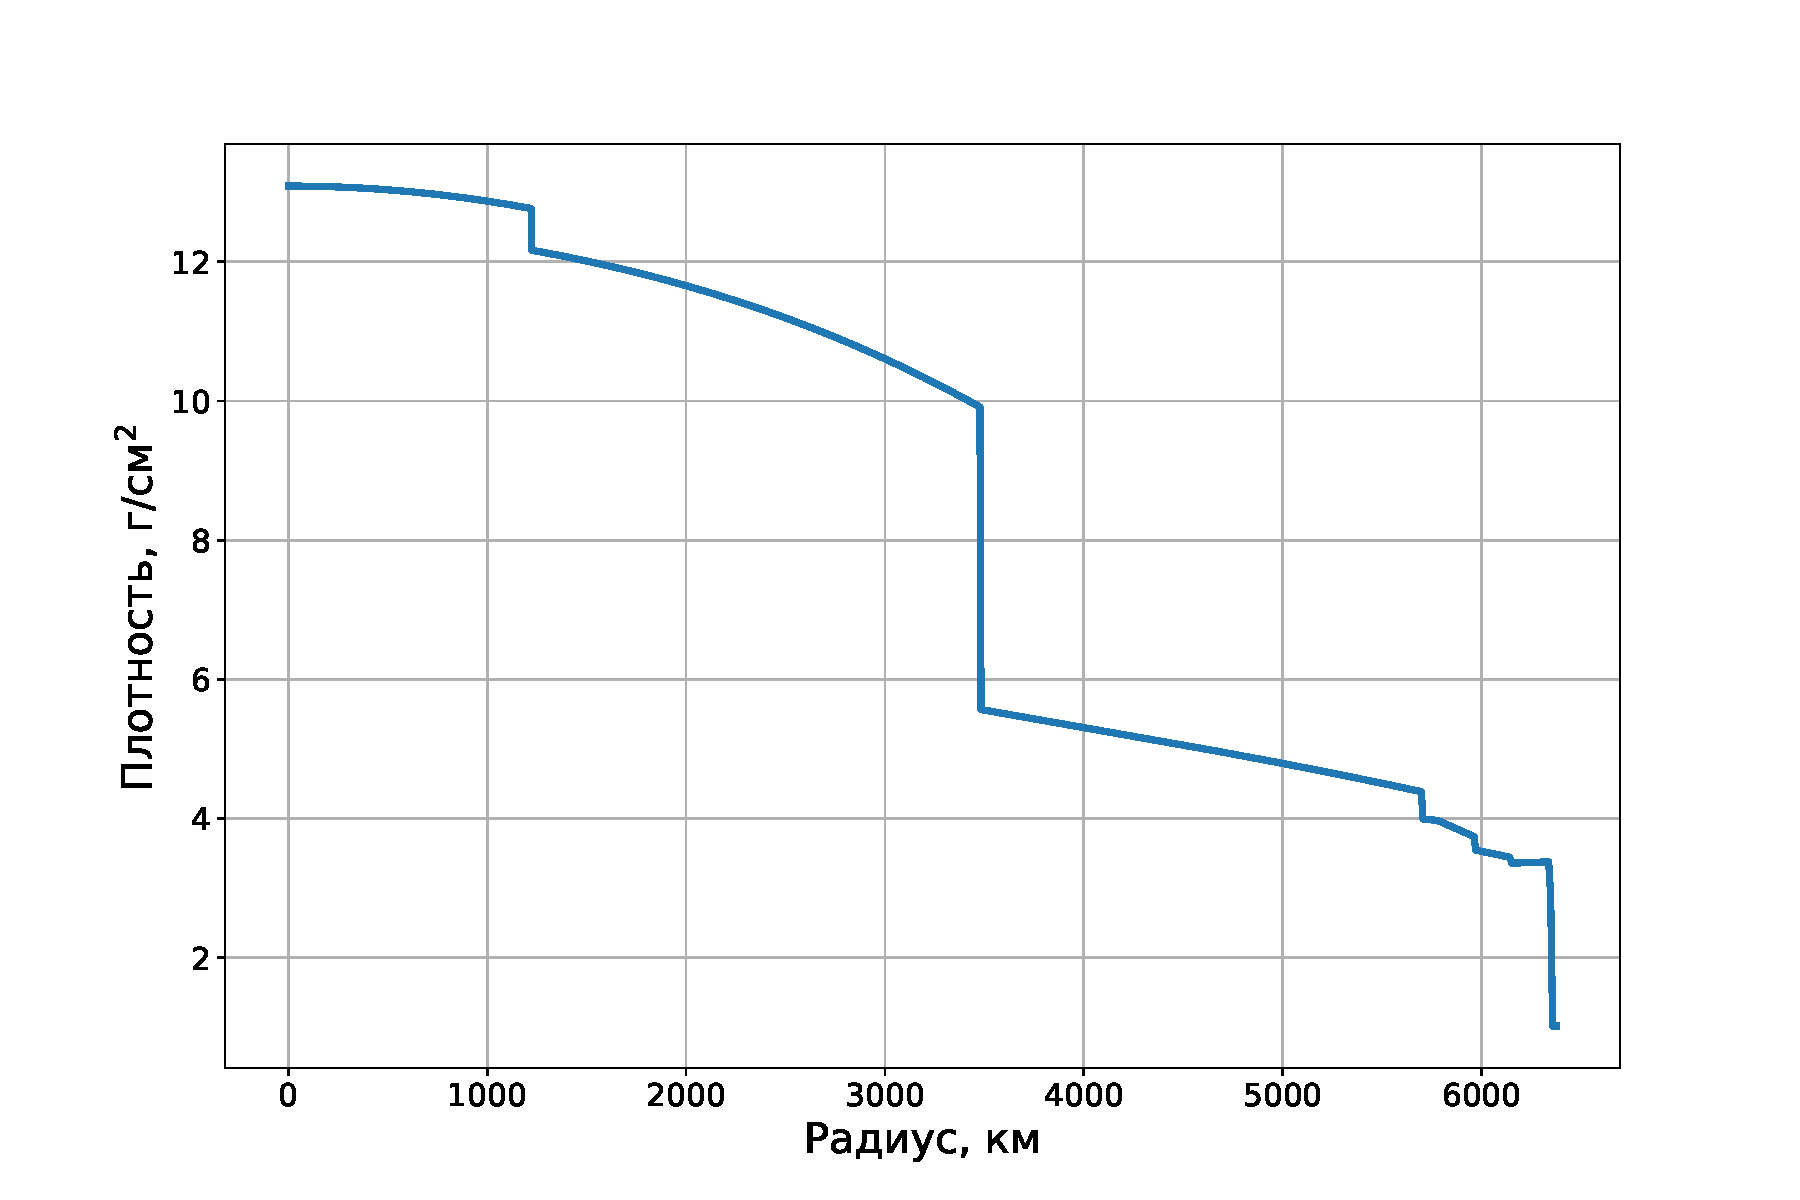
\includegraphics[width=\linewidth]{images/NuProp/PREM.pdf}
\caption{Плотность вещества в модели Земли PREM.}
\label{PREM}
\end{figure}

Расчёт толщины вещества, проходимого нейтрино, осуществляется интегрированием плотности вдоль траектории. Поддерживаются несколько численных методов: метод прямоугольников, квадратурный метод \texttt{quad} из \texttt{SciPy}, и метод Монте-Карло \texttt{vegas}. Изотопный состав вещества задаётся в модуле Earth пакета \texttt{NuPropagator}.

\subsection{Метод Z-фактора}

Z-фактор представляет собой поправку к затуханию потока нейтрино, учитывающую регенерацию за счёт нейтрального тока. Метод подробно описан в работе~\cite{naumov1999} и базируется на решении следующего уравнения переноса нейтрино:
\begin{equation}
\frac{\partial F_{\nu}(x,E)}{\partial x} = \frac{1}{\lambda_{\nu}(E)}\left[ \int\limits_0^1\frac{dy}{1-y}\Phi_{\nu}(y,E) F_{\nu}(x,E_y) - F_{\nu}(x,E) \right],
\end{equation}
где $F_{\nu}(x,E)$ — поток нейтрино после прохождения толщины $x$, $E_y = E/(1-y)$, $\lambda{E}$ - полное сечение взаимодействия нейтрино с веществом, а $\Phi_{\nu}(y,E)$ — распределение по передаче энергии, определяемое следующей формулой:
\begin{equation}
    \Phi_{\nu}(y,E) = \frac{\sum\limits_{T\in \{n,p,e\}}N_T\frac{d\sigma_{\nu T}}{dy}(y,E_y)}{\sum\limits_{T\in \{n,p,e\}}N_T\sigma_{\nu T}(E)}
\end{equation}

Предполагаемое решение имеет вид:
\begin{equation}
F_{\nu}(x,E) = F^{0}_{\nu}(E)\exp\left(-\frac{x}{\Lambda_{\nu}(x,E)}\right),
\end{equation}
где 
\begin{equation}
\Lambda_{\nu}(x,E) = \frac{\lambda_{\nu}(E)}{1 - \mathcal{Z}_{\nu}(x,E)}.
\end{equation}

\subsection{Итерационный метод и его реализация}

Решение уравнения для $Z_{\nu}(x,E)$ реализуется итерационно, начиная с $Z^{(0)}$ и строя следующие приближения по схеме:
\begin{equation}
\mathcal{Z}^{(n+1)}_{\nu}(x,E) = \int\limits_0^x dx' \int\limits_0^1 dy\,\eta_{\nu}(y,E)\Phi_{\nu}(y,E)\exp\left[ -x'D^{(n)}_{\nu}(x',E,E_y) \right],
\end{equation}
где $\eta_{\nu}(y,E)$ — весовой фактор, определяемый формой начального спектра. Точное выражение для $\eta_{\nu}(y,E)$ имеет следующий вид: 
\begin{equation}
    \eta_{\nu}(y,E) = \frac{F^0_{\nu}(E_y)}{(1-y)F^0_{\nu}(E)}.
\end{equation}
Выражение для фактора $D^{(n)}_{\nu}(x, E, E_y)$ имеет следующий вид:
\begin{equation}
    D^{(n)}_{\nu}(x, E, E_y) = \frac{1-\mathcal{Z}_{nu}^{(n)}(x, E_y)}{\lambda(E_y)} - \frac{1-\mathcal{Z}_{nu}^{(n)}(x, E)}{\lambda(E)}
\end{equation}
Реализация учитывает как исчезновение нейтрино за счёт заряженного тока, так и эффект регенерации от нейтрального тока. Конечная плотность потока описывается экспоненциальным затуханием с учётом эффективной длины пробега:
\begin{equation}
P(E,x) = \exp(-x/\lambda_{\nu}(E)), \quad x = \int\rho(l)\,dl.
\end{equation}
\subsection{Сравнение с другими программными пакетами}
В данной главе бкдет проведено сравнение результатов, полученных с помощью двух програмнных пакетов: \texttt{nuFATE}~\cite{Vincent_2017} и \texttt{nupropagator}
\subsection{Дополнительные возможности}
% (Оставьте место для дополнения при необходимости)

\subsection{Интеграция с другими модулями}
% (Добавьте описание связей с другими компонентами симуляционного фреймворка)

\subsection{Поддержка и установка}

Пакет \texttt{NuPropagator} доступен через \texttt{PyPI} и может быть установлен командой:
\begin{verbatim}
pip install nupropagator
\end{verbatim}
Полная документация доступна на странице проекта, включающей примеры использования и описание API.
